\section{Introduction} \label{sec:introduction}

In real-world applications of visual object recognition, performance is time-sensitive.% and inherently tied to the many-class nature of the world.
In robotics, a small finite amount of processing power per unit time is all that is available for robust object detection, if the robot is to usefully interact with humans.
In large-scale detection systems, such as image search, results need to be obtained quickly per image as the number of items to process is constantly growing.
In such cases, an acceptable answer at a reasonable time may be more valuable than the best answer given too late.

\begin{figure}[ht!]
\center{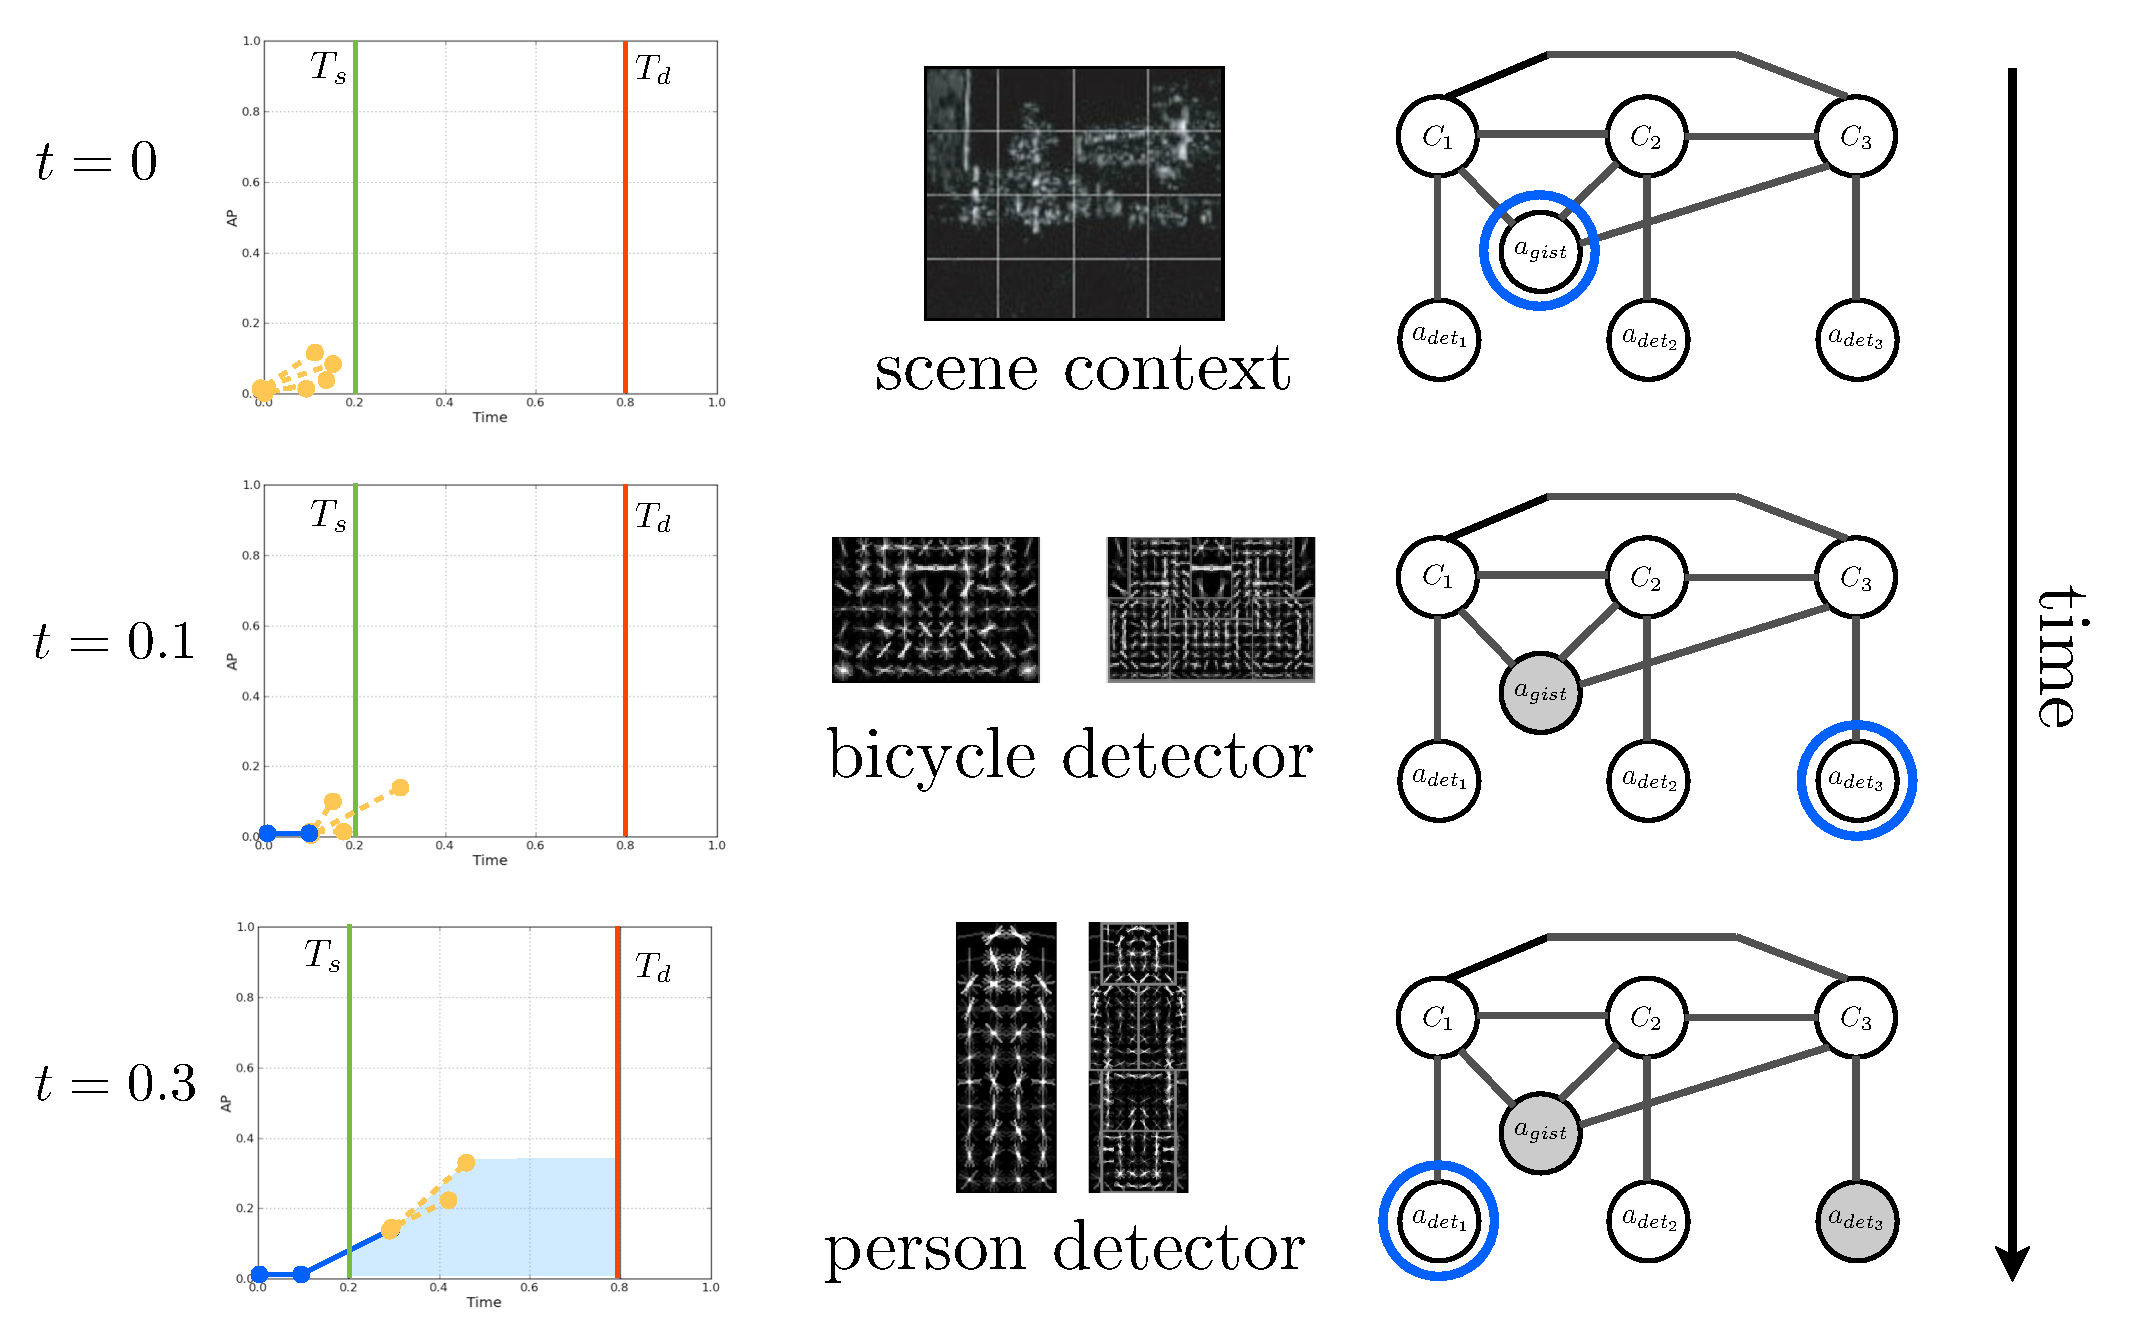
\includegraphics[width=0.86\linewidth]
    {../figures/figure1.pdf}}
  \caption{
A sample trace of our method.
At each time step beginning at $t=0$, potential actions are considered according to their \emph{value}, and the $\arg\max$ action is picked.
The selected action is performed and returns \emph{observations}.
Different actions return different observations: a detector returns a list of detections, while a scene context action simply returns its cmoputed feature. 
The \emph{belief model} of our system is updated with the observations, which influences the selection of the next action.
The final evaluation of a detection episode is the area of the \emph{AP vs. Time curve} between given start and end times.
The value of an action is the expected result of final evaluation if the action is taken and the policy continues to be followed, which allows actions without an immediate benefit to be scheduled.
}
  \label{fig:figure1}
\end{figure}

A hypothetical system for vision-based advertising presents a case study: companies pay money to have their products detected in images on the internet.
The system has different values (in terms of cost per click) and accuracies for different classes of objects, and the queue of unprocessed images varies in size.
The detection strategy to maximize profit in such an environment has to exploit every inter-object context signal available to it, because there is not enough time to run detection for all classes.

What matters in the real world is timeliness, and either not all images can be processed or not all classes can be evaluated in a detection task.
Yet the conventional approach to evaluating visual recognition does not consider efficiency, and evaluates performance independently across classes.
We argue that the key to tackling problems of dynamic recognition resource allocation is to start asking a new question:
\emph{What is the best performance we can get on a budget?}

Taking the task of object detection, we propose a new \emph{timeliness} measure of performance vs. time (shown in Figure~\ref{fig:figure1}).
We present a method that treats different detectors and classifiers as black boxes, and uses reinforcement learning to learn a dynamic policy for selecting actions to achieve the highest performance under this evaluation.
Evaluating on the PASCAL VOC dataset and evaluation regime, we are able to obtain better performance than all baselines when there is less time available than is needed to exhaustively run all detectors.
